\begin{surferPage}[Cúspide A2+-]{Una cúspide (singularitat $A_2^{+-}$)}
L'equació següent correspon a una \emph{cúspide} o
 \emph{singularitat cuspidal}:
    \vspace*{-0.4em}
    \begin{center}
      $x^3+y^2-z^2=0.$
    \end{center}
    \vspace*{-0.4em}
És anàloga a la cúspide de la corba plana obtinguda tallant la
superfície amb un pla. Per exemple, el pla $z=0$ ens dóna la corba
$x^3+y^2=0$:
    \vspace*{-0.7em}
    \begin{center}
      \begin{tabular}{c@{\ }c@{\ }c@{\ }c}
        \begin{tabular}{@{}c@{}}
          
\includegraphics[width=1.2cm]{../../common/images/A2pm}
        \end{tabular}
        &
        \begin{tabular}{@{}c@{}}
          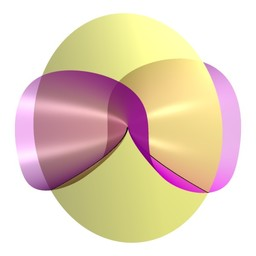
\includegraphics[width=1.2cm]{../../common/images/cuspe_cut}
        \end{tabular}
        &
        \begin{tabular}{@{}c@{}}
          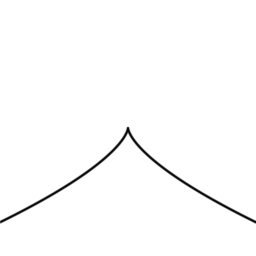
\includegraphics[width=1.2cm]{../../common/images/cuspe_rot}
        \end{tabular}
        &
        \begin{tabular}{@{}c@{}}
          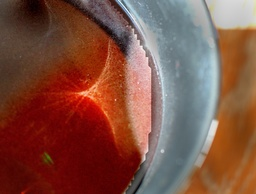
\includegraphics[width=1.4cm]{../../common/images/kuspe_detail_gross_heller}
        \end{tabular}
      \end{tabular}
    \end{center}
    \vspace*{-0.4em}
La imatge a la dreta mostra la cúspide que forma la llum reflectida
en una tassa.

Una singularitat de tipus $A_k^{+-}$ es pot deformar en
    $\lfloor\frac{k+1}{2}\rfloor$
singularitats còniques. En el cas $k=2$, per exemple, la
deformació és
    \[(1-a)x^3+ax^2+y^2-z^2=0.\]
Per a $a=0$, s'obté la cúspide, i per a valors petits de $a\neq0$,
una singularitat cònica:
    \vspace*{-0.6em}
    \begin{center}
      \begin{tabular}{@{}c@{\quad}c@{\quad}c@{}}
        \begin{tabular}{@{}c@{}}
          
\includegraphics[width=1.1cm]{../../common/images/A2pm_0}
        \end{tabular}
        &
        \begin{tabular}{@{}c@{}}
          
\includegraphics[width=1.1cm]{../../common/images/A2pm_1}
        \end{tabular}
        &
        \begin{tabular}{@{}c@{}}
          
\includegraphics[width=1.1cm]{../../common/images/A2pm_2}
        \end{tabular}
      \end{tabular}
    \end{center}
 
\end{surferPage}
